\subsection{Experiment}

As a way to test our hypothesis we conducted a behavioral experiment to gather empirical data. We developed a web app where people could participate in a simulated investment task.

In the experiment people where told that they own a house that they want to sell. At the beginning of the simulation the housing market is in recession but when the participants wait long enough it will eventually change to a booming market and prices will increase. To introduce pressure on the participants they have to pay maintenance cost for every year they wait.
The goal then is to sell the house as soon as possible after the market has become booming.

The current state of the market is not directly observable by the participant. Instead at each time step one of the following things was shown to them:
\begin{itemize}
    \item Scenario 1: a price for which one of the houses in their neighborhood was sold, samples from a gaussian distribution with different mean depending on the market state.
    \item Scenario 2: the belief of an "expert" (the Bayesian estimate based on the observation history) that shows the chances of the market being in a good state
\end{itemize}

Given this information they had to infer in what state the market actually is and act accordingly.

~\autoref{fig:user-interface} shows how the interface of the experiment looked like for the two scenarios. In the first scenario, the participant was shown a new house price together with all the past observations in the form of a historic plot. In the second scenario they were given only the current belief. Besides this the interface constantly shows the total amount of money that the participant has spent on maintenance so far.

\begin{figure}[!htbp]
    \centering
    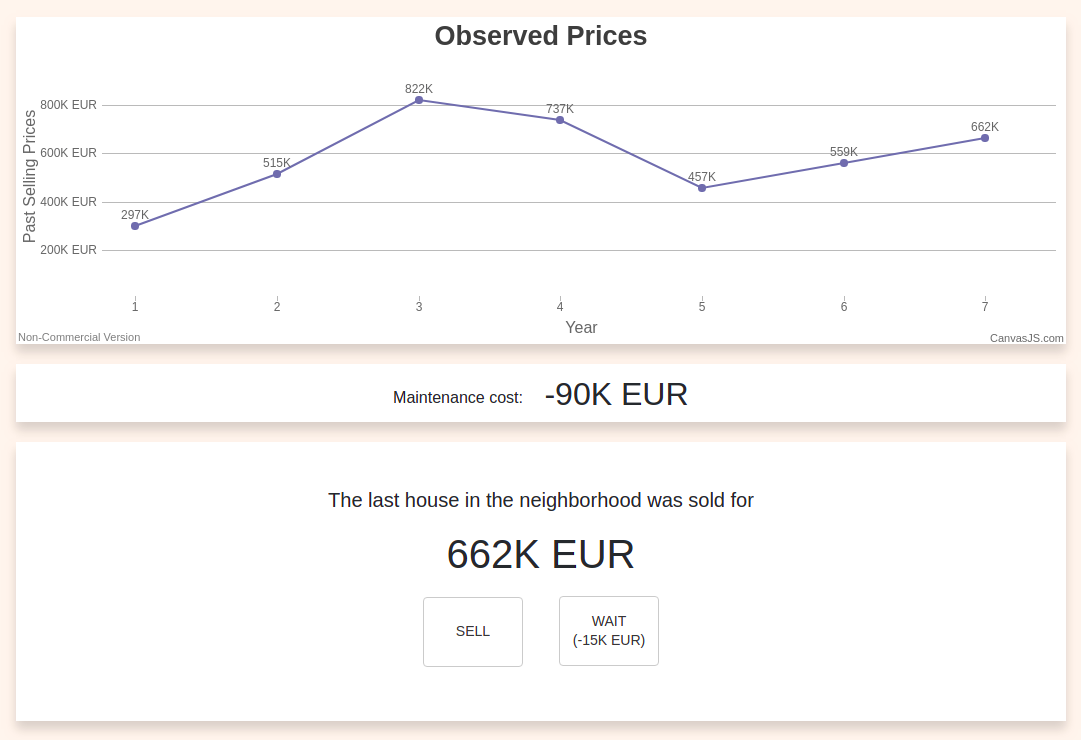
\includegraphics[width=0.99\linewidth]{img/methods/experiment_obs_1.png}\\
    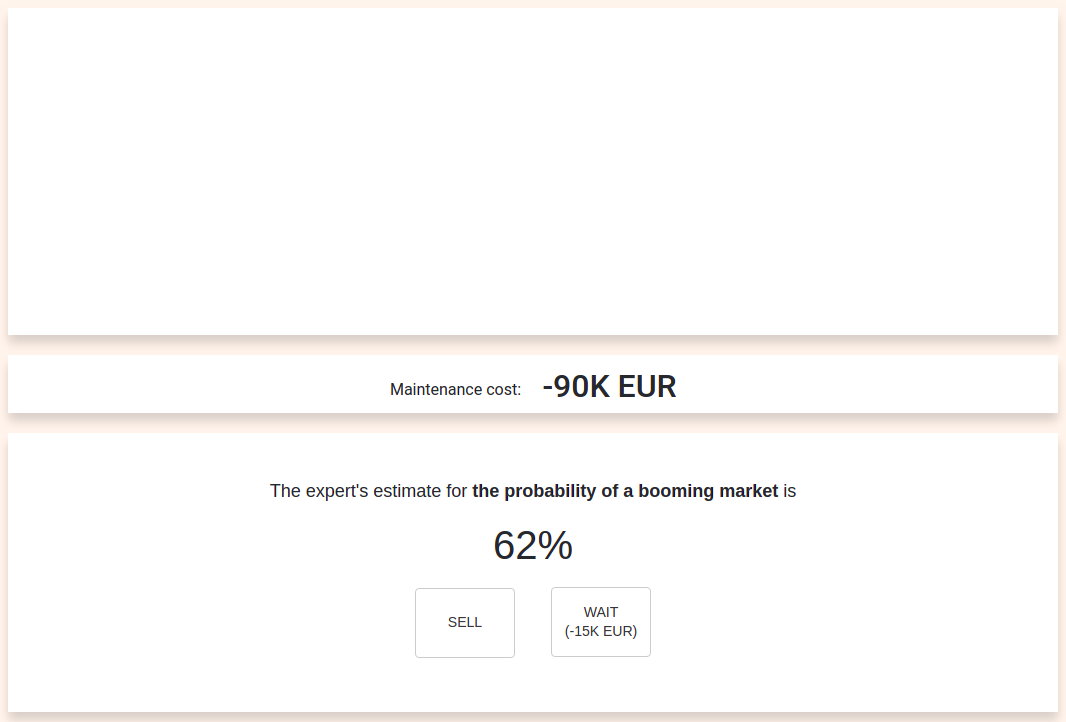
\includegraphics[width=0.99\linewidth]{img/methods/experiment_bel_1.png}\\
    \caption{The two experiment scenarios and their respective UI. In (a) subjects are shown the observation history at the top and a new observation at the bottom. In (b) they see the Bayesian estimate based on the observation history.}\label{fig:user-interface}
\end{figure}

~\autoref{fig:states} shows a graphical representation of the underlying environment. The market has three states, \textit{recession}, \textit{booming} and \textit{sold}. The market starts in recession in each experiment and iteratively transitions are performed. At each transition subjects are shown an observation from the current state and can choose between \textit{wait} and \textit{sell}. The experiments ends when subjects sell and they receive a reward based on the last market state.

\begin{figure}[H]
\tikzset{
scale=0.62, every node/.append style={transform shape}
}
\begin {center}
\begin {tikzpicture}[-latex ,auto ,node distance =3cm and 4cm ,on grid ,
semithick , scale=0.5, transform shape,
state/.style ={ circle ,fill=black!20, minimum width =3 cm}]
\node[state] (C){\large Sold};
\node[state] (A) [above left=of C,align=center] {\large Recession};
\node[state] (B) [above right =of C,align=center] {\large Booming};
\coordinate[below of=A] (AA);
\coordinate[below of=B] (BB);
\coordinate[below of=AA] (D);
\coordinate[below of=BB] (E);

\path (A) edge [loop left, line width=1mm, align=center] node[left] {\large wait \\ $\alpha =$ \\  $0.86$} (A);
\path (A) edge [bend left = -25,line width=1mm,align=center] node[below =0.25 cm] {\large sell\\$1.0$} (C);
\path (A) edge [bend left =25,line width=1mm,align=center] node[above] {\large wait\\$0.14$} (B);

\path (B) edge [loop right,line width=1mm,align=center] node[right] {\large wait\\$1.0$} (B);
\path (B) edge [bend right = -25,line width=1mm,align=center] node[below =0.25 cm] {\large sell\\$1.0$} (C);

%\fill[gray!40!white, opacity=0.5] (-6,-1) rectangle (5,6);

\path (A) edge [bend right =25,line width=1mm, dashed] node[left] {\large $Observation$} (D);
\path (B) edge [bend left  =25,line width=1mm, dashed] node[right] {\large $Observation$} (E);
\end{tikzpicture}
\end{center}
    \caption{Market States}\label{fig:states}
\end{figure}

The experiment was conducted with 24 participants and each one of them did the following runs:
\begin{itemize}
    \item 25 runs with random samples from the observations experiment with an easy setup (low maintenance costs.)
    \item 25 runs with random samples from the observations experiment with a hard setup (high maintenance costs.)
    \item 60 runs with random samples from the belief experiment.
\end{itemize}

The participants were paid according to their performance (average reward over all experiment runs) in order to give motivate them for performing as good as possible in the experiment.